%%%%%%%%%%%%%%%%%%%%%%%%%%%%%%%%%%%%%%%%%%%%%%%%%%%%%%%%%%%%
% LaTeX poster template
% Created by Salma Rodriguez
% Original Template by Nathaniel Johnston
% August 2009
% http://www.nathanieljohnston.com/2009/08/latex-poster-template/
%%%%%%%%%%%%%%%%%%%%%%%%%%%%%%%%%%%%%%%%%%%%%%%%%%%%%%%%%%%%

\documentclass[final]{beamer}
\usepackage[orientation=portrait,size=a0,scale=1.24]{beamerposter}
\usepackage{graphicx}			% allows us to import images
\usepackage[noend]{algpseudocode}

%-----------------------------------------------------------
% Define the column width and poster size
% To set effective sepwid, onecolwid and twocolwid values, first choose
% how many columns you want and how much separation you want between columns
% The separation I chose is 0.024 and I want 4 columns
% Then set onecolwid to be (1-(4+1)*0.024)/4 = 0.22
% Set twocolwid to be 2*onecolwid + sepwid = 0.464
%-----------------------------------------------------------

\newlength{\sepwid}
\newlength{\onecolwid}
\newlength{\twocolwid}
\setlength{\sepwid}{0.016\paperwidth}
\setlength{\onecolwid}{0.312\paperwidth}
\setlength{\twocolwid}{0.64\paperwidth}
\setlength{\topmargin}{-0.5in}
\usetheme{confposter}
\usetheme{headline}
\usepackage{exscale}

\graphicspath{{../images/}}

%-----------------------------------------------------------
% The next part fixes a problem with figure numbering. Thanks Nishan!
% When including a figure in your poster, be sure that the commands are typed in the following order:
% \begin{figure}
% \includegraphics[...]{...}
% \caption{...}
% \end{figure}
% That is, put the \caption after the \includegraphics
%-----------------------------------------------------------

\usecaptiontemplate{
    \small
    \structure{\insertcaptionname~\insertcaptionnumber:}
\insertcaption}

%-----------------------------------------------------------
% Define colours (see beamerthemeconfposter.sty to change these colour definitions)
%-----------------------------------------------------------

\setbeamercolor{block title}{fg=ngreen,bg=white}
\setbeamercolor{block body}{fg=black,bg=white}
\setbeamercolor{block alerted title}{fg=white,bg=dblue!70}
\setbeamercolor{block alerted body}{fg=black,bg=dblue!10}

\setbeamerfont{footline}{size=\large,series=\tt}

% \begin{beamercolorbox}[wd=\paperwidth]{lower separation line head}
%   \rule{0pt}{2pt}
% \end{beamercolorbox}
% 

%-----------------------------------------------------------
% Name and authors of poster/paper/research
%-----------------------------------------------------------

\title{SSD-based Energy Efficient Cloud Storage}

\author{Salma Rodriguez}
\institute{Florida International University \\
       Mentor: Prof. Ming Zhao, VISA Laboratory \\
       Instructor: Masoud Sadjadi}

%-----------------------------------------------------------
% Start the poster
%-----------------------------------------------------------

\begin{document}
\begin{frame}[t]
    \begin{columns}[t]												% the [t] option aligns the column's content at the top
	\begin{column}{\sepwid}\end{column}			% empty spacer column
	\begin{column}{\onecolwid}
	    \begin{alertblock}{Problem Statement}
		Can we save power in storage servers by spinning down
		the disk dynamically while caching data on solid state drives?
	    \end{alertblock}
	    \vskip2ex
	    \setbeamercolor{block alerted body}{fg=black,bg=white}
	    \begin{alertblock}{Motivation}
		\begin{block}
		    {Solid State Technology}
		    High capacity EEPROM devices have been shown to
		    reduce energy consumption when used
		    as local cache for hard disk drives. %\cite{key2,key3}.
		\end{block}
		\vskip2ex
		\begin{block}
		    {Distributed SSD Caching}
		    With our caching solution, we hope to increase
		    the working set in flash memory and keep server disks spun down.
		\end{block}
		\vskip2ex
		\begin{block}
		    {Properties to Explore}
		    We explore the properties of dynamic spin down of storage
		    server disks.
		\end{block}
	    \end{alertblock}
	    \vskip2ex
	    \begin{block}{Linux Device Mapper}
	        %\begin{tabular}{m{0.465\linewidth}m{0.465\linewidth}}
	        	%\hline
	        \begin{itemize}
	            \item Device Mapper facilitates mapping between two block devices.
	            \item Only pseudo device in volatile memory is visible to applications.
	            \item Kernel module uses device mapper to map block I/Os sent to pseudo
	        	device onto real devices (source and target).
	            \item Devices may not necessarily be locally attached.
	        \end{itemize} %&
	        \begin{figure}
	            %\caption{Device Mapper Layout}
	            \centering 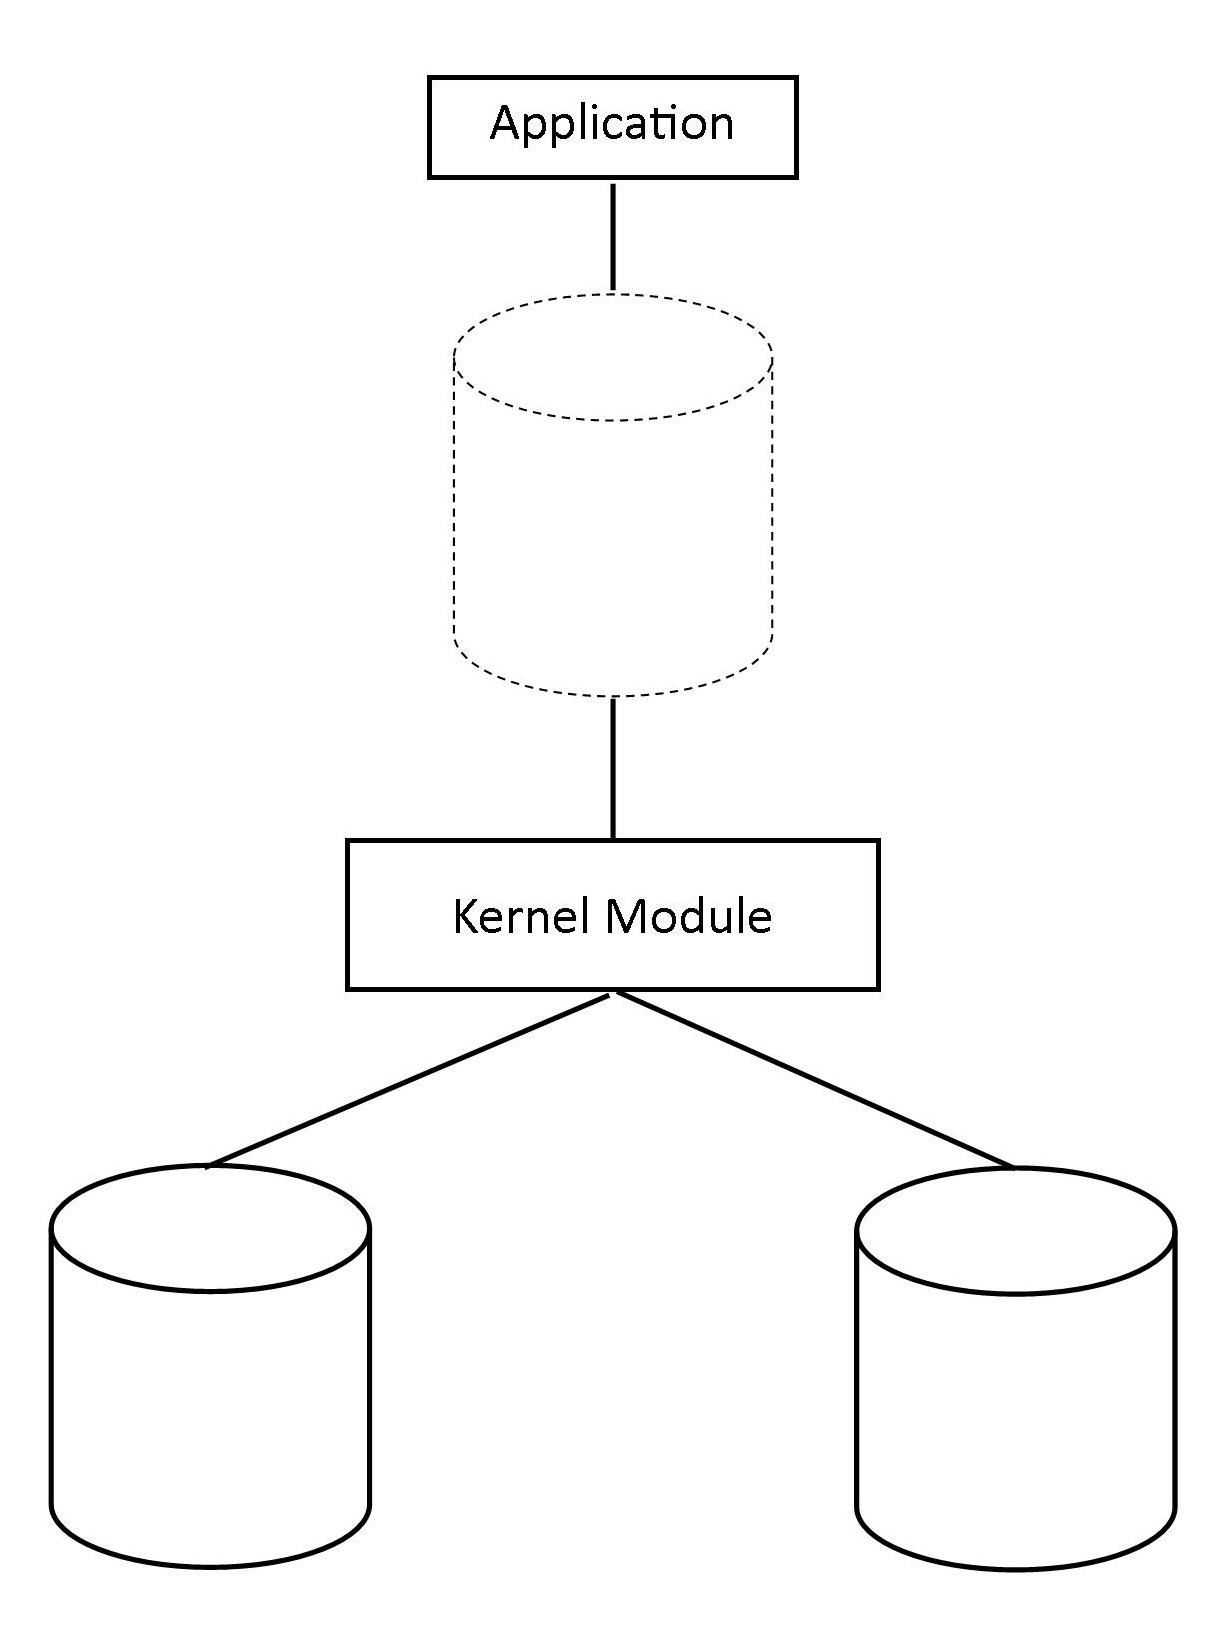
\includegraphics[scale=1]{DM.jpg}
	            \label{fig:dm}
	        \end{figure} %\\
	        	%\hline
	            %\end{tabular}
	    \end{block}
	\end{column}
	\begin{column}{\sepwid}\end{column}
	\begin{column}{\twocolwid}
	    \setbeamercolor{block alerted body}{fg=black,bg=white}
	    \begin{alertblock}{Spin Down Policy}
		\begin{column}{\onecolwid}
		    \begin{block}{Design}
			\raggedright Dynamic spin down policy for Device Mapper Cache (DM Cache)
			    Keep server disks (source device) spun down when cache is bigger \\
			    than the working set. \\
			\vspace{15pt}
			\raggedright Figure 1: The state of each disk is controlled dynamically.
			\vspace{15pt}
			\begin{figure}
			    \centering 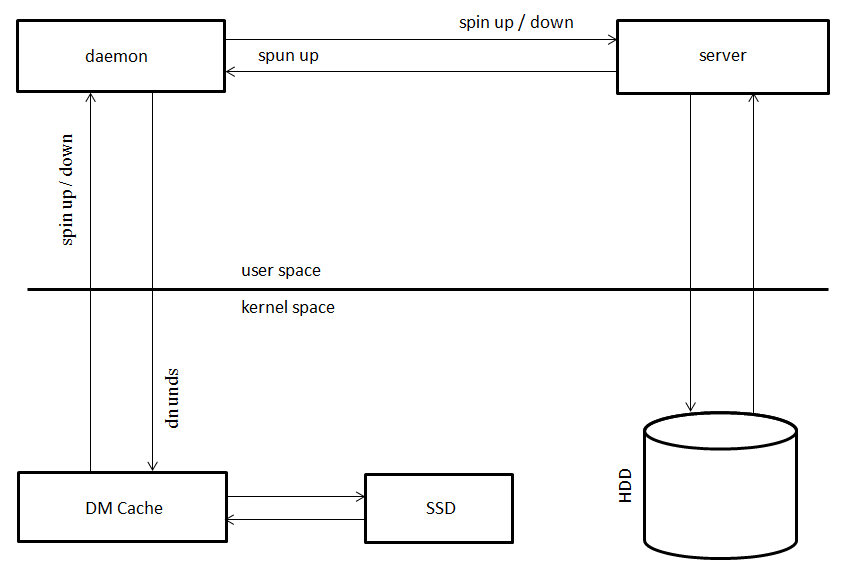
\includegraphics{drawing.png}
			    \label{fig:struct}
			\end{figure}
		    \end{block}
		\end{column}
		\begin{column}{\onecolwid}
		    \begin{block}{Implementation}
			\bf Algorithm 1 \rm spinning the disk up or down dynamically \\
			\algrenewcommand\algorithmicrequire{\textbf{Precondition:}}
			\begin{algorithmic}[1]
			    \Require{server disk is spinning}
			    \Procedure{Spin Up or Down}{}
			    \State $T\gets$ constant time
				\While{true}
				    \State sleep for $T$ seconds
				    \If{disk is spinning}
					\State $k\gets$ current time in sec
					\State $c\gets$ last cache miss
					\If{$c$ + $T \leq k$}
					    \State spin down the disk
					    \State $\text{state}\gets \text{not spinning}$
					\EndIf
				    \Else \Comment{disk is not spinning}
					\If{blocking}
					    \State spin up the disk
					    \State $\text{state} \gets \text{spinning}$
					    \State unblock DM Cache
					\EndIf
				    \EndIf
				\EndWhile
			    \EndProcedure
			\end{algorithmic}
		    \end{block}
		\end{column}
	    \end{alertblock}
	    \vskip2ex
	    \begin{block}{Evaluation}
		The baseline for our results is a simple iSCSI storage setup.
		We ran a 30 min test using a webserver-based workload, and
		observed that context switches increase power by 14W more than the baseline.
	    \end{block}
	    \begin{columns}[t,totalwidth=\twocolwid]
		\begin{column}{\onecolwid}
		    %\setbeamercolor{block alerted title}{fg=black,bg=norange}
		    \begin{block}{Spin Down with Schedule}
			\begin{figure}
			    \raggedright Figure 2: Red plot: DM Cache with spin down daemon. Blue Plot:
				iSCSI without DM Cache. \\
			    \vspace{15pt}
			    \centering 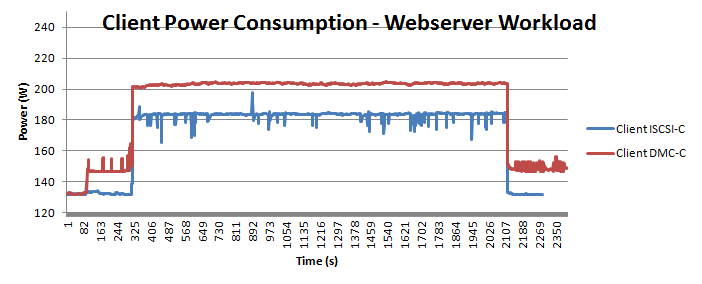
\includegraphics[scale=1.35]{image.png}
			    \label{fig:results}
			\end{figure}
		    \end{block}
		\end{column}
		\begin{column}{\onecolwid}
		    \begin{block}{Spin Down with Sleep}
			\begin{figure}
			    \raggedright Figure 3: Red plot: DM Cache with spin down daemon. Blue Plot:
			    iSCSI without DM Cache. \\
			    \vspace{15pt}
			    \centering 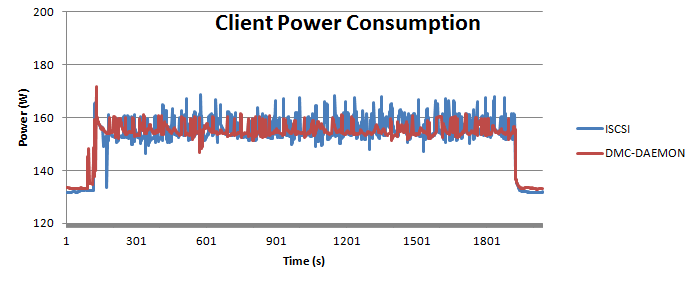
\includegraphics[scale=1.35]{image2.png}
			    \label{fig:results}
			\end{figure}
		    \end{block}
		\end{column}
	    \end{columns}
	    \vskip2ex
	    \begin{alertblock}{Spin Down Results for Server}
		\begin{figure}
		    \raggedright Figure 4: Spin down daemon reduces power on storage server. \\
		    \vspace{15pt}
		    \centering 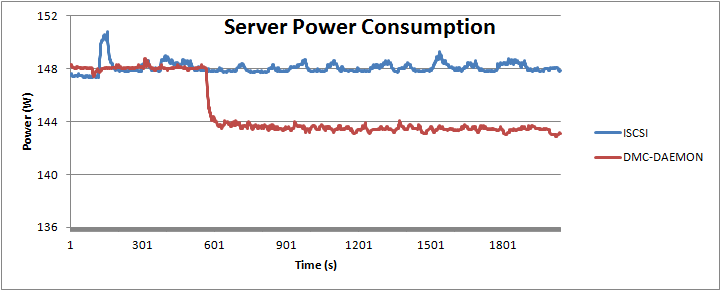
\includegraphics[width=0.7\linewidth]{image3.png}
		    \label{fig:results}
		\end{figure}
	    \end{alertblock}
	\end{column}
	\begin{column}{\sepwid}\end{column}			% empty spacer column
    \end{columns}
    \vskip2ex
    \begin{block}{Acknowledgements}
	I extend my gratitude to Jorge Cabrera for assisting me with the
	benchmarks and the shell
	scripts that allow the spin down daemon to interact with the disks on the storage server. I
	am also thankful to Jesus Ramos for pointing out the "grammar squiggles" in my draft of
	figure 1.
    \end{block}
\end{frame}
\end{document}
